\documentclass[preprint]{../common/sigplanconf}

\usepackage{amsmath}
%\usepackage{amsthm}
\usepackage{url}
\usepackage{graphicx}

\usepackage{tikz}
\usepackage{tkz-graph}
\usetikzlibrary{arrows}
\usetikzlibrary{fit}					% fitting shapes to coordinates
\usetikzlibrary{backgrounds}	% drawing the background after the foreground
\usetikzlibrary{arrows}

\usepackage{color}
\definecolor{Red}{rgb}{0.9,0.0,0.0}  % fixme
\definecolor{Green}{rgb}{0.0,0.4,0.0}
\definecolor{Blue}{rgb}{0.0,0.0,0.9}
\definecolor{DarkBlue}{rgb}{0.0,0.0,0.75}
\definecolor{Midnight}{rgb}{0.0,0.0,0.5}
\definecolor{Purple}{rgb}{0.5,0.0,0.4}
\definecolor{Black}{rgb}{0.0,0.0,0.0}
\definecolor{Yellow}{rgb}{1.0,1.0, 0.25}
\definecolor{Cyan}{rgb}{0.25,1.0, 1.0}

\newcommand{\cdColor}{Black}
\newcommand{\kwColor}{DarkBlue}
\newcommand{\comColor}{Red}

\usepackage{listings}
\lstdefinelanguage{Rust}[]{C}{%
  morekeywords={abstract,alignof,as,become,box,break,const,continue,crate,do,enum,extern,false,
  final,fn,for,if,impl,in,let,loop,macro,match,mod,move,mut,offsetof,override,priv,pub,pure,ref,return,
  sizeof,static,self,struct,super,true,trait,type,typeof,unsafe,unsized,use,virtual,where,while,yield},
  % otherkeywords={(|,|),[|,|],(,),[,],\{,\},\,,:,...,_,|,=,=>,->,\#,:>},
  otherkeywords={::,->,\#},
}[keywords,comments,strings]%

\lstset{
  basicstyle=\ttfamily\color{\cdColor},
  keywordstyle=\color{\kwColor}\bfseries,
  commentstyle=\color{\comColor}\itshape,
  language=Rust
}

\newcommand{\dcfa}{{$\Delta$}{CFA}}
\newcommand{\gcfa}{{$\Gamma$}{CFA}}

\usepackage{algorithm}
\usepackage{algpseudocode}

% common LaTeX macros
%
% Last modified: 04-07-2010
%

\usepackage{times}
%-------------------------
% the following magic makes the tt font in math mode be the same as the
% normal tt font (i.e., Courier)
%
\SetMathAlphabet{\mathtt}{normal}{OT1}{pcr}{m}{n}
\SetMathAlphabet{\mathtt}{bold}{OT1}{pcr}{bx}{n}
%-------------------------

\usepackage{amsmath}
\usepackage{amssymb} % for \pitchfork

\newcommand{\NOTE}[1]{%
  \par\leavevmode\noindent\textbf{[[ #1 ]]}\par\leavevmode\noindent}
\newcommand{\CUT}[1]{}
\newcommand{\SIDENOTE}[1]{%
  \marginpar{\tiny\raggedright{#1}}}

\newcommand{\algoref}[1]{Algorithm~\ref{#1}}
\newcommand{\appref}[1]{Appendix~\ref{#1}}
\newcommand{\chapref}[1]{Chapter~\ref{#1}}
\newcommand{\secref}[1]{Section~\ref{#1}}
\newcommand{\tblref}[1]{Table~\ref{#1}}
\newcommand{\figref}[1]{Figure~\ref{#1}}
\newcommand{\listingref}[1]{Listing~\ref{#1}}
\newcommand{\pref}[1]{{page~\pageref{#1}}}
\newcommand{\defref}[1]{Definition~\ref{#1}}
\newcommand{\ruleref}[1]{Rule~\ref{#1}}

\newcommand{\eg}{{\em e.g.}}
\newcommand{\cf}{{\em cf.}}
\newcommand{\ie}{{\em i.e.}}
\newcommand{\etc}{{\em etc.\/}}
\newcommand{\naive}{na\"{\i}ve}
\newcommand{\Naive}{Na\"{\i}ve}
\newcommand{\ala}{{\em \`{a} la\/}}
\newcommand{\etal}{{\em et al.\/}}
\newcommand{\role}{r\^{o}le}
\newcommand{\vs}{{\em vs.}}
\newcommand{\forte}{{fort\'{e}\/}}

%
% language names
\newcommand{\Cplusplus}{\mbox{C\hspace{-.05em}\raisebox{.4ex}{\tiny\bf ++}}}
\newcommand{\Cmm}{\mbox{C\hspace{-.05em}\raisebox{.4ex}{\small\textbf{{-}{-}}}}}
\newcommand{\csharp}{\textsc{C\#}}
\newcommand{\C}{\textsc{C}}
\newcommand{\Ckit}{\textsc{Ckit}}
\newcommand{\java}{\textsc{Java}}
\newcommand{\ghc}{\textsc{GHC}}
\newcommand{\loom}{\textsc{Loom}}
\newcommand{\moby}{\textsc{Moby}}
\newcommand{\minimoby}{\textsc{MiniMoby}}
\newcommand{\micromoby}{\textsc{microMoby}}
\newcommand{\MOC}{\textsc{MOC}}
\newcommand{\ml}{\textsc{ML}}
\newcommand{\nesl}{{\textsc{Nesl}}}
\newcommand{\sml}{\textsc{SML}}
\newcommand{\smlnj}{\textsc{SML/NJ}}
\newcommand{\mlj}{\textsc{MLj}}
\newcommand{\cml}{\textsc{CML}}
\newcommand{\pml}{\textsc{PML}}
\newcommand{\ocaml}{\textsc{OCaml}}
\newcommand{\mlkk}{\textsc{ML2000}}
\newcommand{\haskell}{\textsc{Haskell}}
\newcommand{\mltwok}{\textsc{ML2000}}
\newcommand{\scala}{\textsc{Scala}}
\newcommand{\perl}{\textsc{Perl}}
\newcommand{\scheme}{\textsc{Scheme}}
\newcommand{\unix}{\textsc{Unix}}
\newcommand{\smalltalk}{\textsc{Smalltalk}}
\newcommand{\self}{\textsc{Self}}
\newcommand{\sting}{\textsc{Sting}}
\newcommand{\parlisp}{\textsc{Paralation Lisp}}
\newcommand{\nkl}{\textsc{Nkl}}
\newcommand{\fkl}{\textsc{Fkl}}
\newcommand{\dkl}{\textsc{Dkl}}

%
% font commands
\providecommand{\bftt}[1]{{\ttfamily\bfseries{}#1}}
\providecommand{\ittt}[1]{{\ttfamily\itshape{}#1}}
\providecommand{\kw}[1]{\bftt{#1}}
\providecommand{\nt}[1]{{\rmfamily\itshape{#1}}}
\providecommand{\term}[1]{{\sffamily{#1}}}
\providecommand{\tyvar}[1]{\ittt{#1}}
%
% math-mode versions
\providecommand{\mkw}[1]{\ensuremath{\text{\kw{#1}}}}
\providecommand{\mnt}[1]{\ensuremath{\text{\nt{#1}}}}
\providecommand{\mterm}[1]{\ensuremath{\text{\term{#1}}}}
\providecommand{\mtyvar}[1]{\ensuremath{\text{\tyvar{#1}}}}

% braces (in math mode)
\newcommand{\LCB}{\mkw{\{}}
\newcommand{\RCB}{\mkw{\}}}

% underscore
\newcommand{\US}{\char`\_}

%%%%%
% Some common math notation
%

% double brackets
\newcommand{\LDB}{\ensuremath{[\mskip -3mu [}}
\newcommand{\RDB}{\ensuremath{]\mskip -3mu ]}}

\newcommand{\dom}{\ensuremath{\mathrm{dom}}}
\newcommand{\rng}{\ensuremath{\mathrm{rng}}}

% sets
\newcommand{\SET}[1]{\ensuremath{\{#1\}}}
\newcommand{\Fin}{\textrm{Fin}}     % finite power set
\newcommand{\DISJOINT}[2]{\ensuremath{#1 \pitchfork #2}}
\newcommand{\finsubset}{\mathrel{\stackrel{\textrm{fin}}{\subset}}}


% finite maps
\newcommand{\finmap}{\mathrel{\stackrel{\textrm{fin}}{\rightarrow}}}
\newcommand{\MAP}[2]{\SET{#1 \mapsto #2}}
\newcommand{\EXTEND}[2]{\ensuremath{#1{\pm}#2}}
\newcommand{\EXTENDone}[3]{\EXTEND{#1}{\MAP{#2}{#3}}}
\newcommand{\SUBST}[3]{\ensuremath{#1[#2\mapsto{}#3]}}
\newcommand{\SUBSTTWO}[5]{\ensuremath{#1[#2\mapsto{}#3,#4\mapsto{}#5]}}


% timestamp
\newcount\timeHH
\newcount\timeMM
\timeHH=\time
\divide\timeHH by 60
\timeMM=\time
\count255=\timeHH
\multiply\count255 by -60 \advance\timeMM by \count255
\newcommand{\timestamp}{%
  \today{} ---
  \ifnum\timeHH<10 0\fi\number\timeHH\,:\,\ifnum\timeMM<10 0\fi\number\timeMM}

\newcommand{\superbeta}{Super-\ensuremath{\beta{}} }

\usepackage{../common/code}


\title{Experience Report: Developing the Servo Web Browser Engine using Rust}

\authorinfo{%
  Lars Bergstrom
}{%
  Mozilla Research}{%
  larsberg@mozilla.com}
\CUT{
  \authorinfo{Matthew Fluet \\
  Matthew Le
}{%
  Rochester Institute of Technology}{%
  \{mtf,ml9951\}@cs.rit.edu}
\authorinfo{%
  John Reppy \\
  Nora Sandler \\
}{%
  University of Chicago}{%
  \{jhr,nlsandler\}@cs.uchicago.edu}
}

\date{\today}

\begin{document}

\maketitle
\thispagestyle{empty}

\sloppy

%!TEX root = paper.tex
%
\begin{abstract}
Inlining is an optimization that replaces a call to a function with that function's 
body.
This optimization not only reduces the overhead of a function call, but can 
expose additional optimization opportunities to the compiler, such as removing
redundant operations or unused conditional branches.
Another optimization, copy propagation, replaces a redundant copy of a still-live 
variable with the original.
Copy propagation can reduce the total number of live variables, reducing register
pressure and memory usage, and possibly
eliminating redundant memory-to-memory copies.
In practice, both of these optimizations are implemented in nearly every
modern compiler.

These two optimizations are practical to implement and effective in first-order 
languages, but in languages with lexically-scoped first-class functions (aka, closures), these optimizations 
are not available to code programmed in a higher-order style.
With higher-order functions, the analysis challenge has been that the 
environment at the call site must be the same as at the closure capture location, 
up to the free variables, or the meaning of the program may change.
Olin Shivers' 1991 dissertation called this family of optimizations 
\emph{\superbeta} and he proposed one analysis technique, called \emph{reflow},
to support these optimizations.
Unfortunately, reflow has proven too expensive to implement in practice.
Because these higher-order optimizations are not available in functional-language
compilers, programmers studiously avoid uses of 
higher-order values that cannot be optimized (particularly in compiler
benchmarks).

This paper provides the first practical and effective technique for 
\superbeta (higher-order) inlining and copy propagation, which
we call unchanged variable analysis.
We show that this technique is practical by implementing it in the 
context of a real compiler for an ML-family language and showing 
that the required analyses have costs below 3\% of the total 
compilation time.
This technique's effectiveness is shown through a set of benchmarks
and example programs, where this analysis exposes additional potential
 optimization sites.
\end{abstract}

%!TEX root = paper.tex
\section{Introduction}
\label{sec:intro}
The heart of a modern web browser is the browser engine, which is the code responsible
for loading, processing, evaluating, and rendering web content.
There are three major browser engine families:
\begin{enumerate}
\item Trident/Spartan, the engine in Internet Explorer~\cite{IE}
\item Webkit\cite{WEBKIT}/Blink, the engine in Safari~\cite{SAFARI}, Chrome~\cite{CHROME}, and Opera~\cite{OPERA}
\item Gecko, the engine in Firefox~\cite{FIREFOX}
\end{enumerate}
All of these engines have at their core many millions of lines of \Cplusplus{} code.
While the use of \Cplusplus{} has enabled all of these browsers to achieve excellent sequential
performance on a single web page, on mobile devices with lower processor speed but many
more processors, these browsers do not provide the same level of interactivity that they
do on desktop processors~\cite{parallelizing-web-pages,ZOOMM}.
Further, in an informal inspection of the critical security bugs in Gecko, we determined that
roughly 50\% of the bugs are use after free, out of range access, or related to integer
overflow.
The other 50\% is split between errors in tracing values from the JavaScript heap in the
\Cplusplus{} code and errors related to dynamically compiled code.

Servo~\cite{SERVO} is a new web browser engine designed to address the major environment and 
architectural changes over the last decade.
The goal of the Servo project is to produce a browser that enables new applications to be authored
against the web platform that run with more safety, better performance, and better power usage
than in current browsers.
To address memory-related safety issues, we are using a new systems programming language,
Rust~\cite{RUST}.
For parallelism and power, we scale across a wide variety of hardware by building either data-
or task-parallelism, as appropriate, into each part of the web platform.
Additionally, we are improving concurrency by reducing the simultaneous access to data
structures and using a message-passing architecture between components such as the
JavaScript engine and the rendering engine that paints graphics to the screen.
Servo is currently over 300k lines of code and implements enough of the web to render and
process many pages, though it is still a far cry from the over 7 million lines of code in
the Mozilla Firefox browser and its associated libraries.
However, we believe that we have implemented enough of the web platform to provide an
early report on the successes, failures, and open problems remaining in Servo, from the
point of view of programming languages and runtime research.
In this experience report, we discuss the design and architecture of a modern web 
browser engine, show how modern programming language techniques --- many of which
originated in the functional programming community --- address these design 
constraints, and also touch on ongoing challenges and areas of research where we
would welcome additional community input.

%%% Local Variables: 
%%% mode: latex
%%% TeX-master: "paper"
%%% End: 

%!TEX root = paper.tex

\section{Browsers}
\label{sec:browsers}

Modern web browsers do not just load static pages, but can also handle pages that have similar
complexity to native applications.
From application suites such as the Google Apps\footnote{\url{https://apps.google.com}} to games
based on the Unreal Engine\footnote{\url{https://www.unrealengine.com/}},
modern browsers have the ability to handle much more than simple static pages.
\figref{fig:browser} shows the steps in processing a site.
While the naming is specific to the Servo browser, similar steps are used in all modern browsers.\footnote{\url{http://www.html5rocks.com/en/tutorials/internals/howbrowserswork/}}
\begin{figure*}[ht]
  \begin{center}
    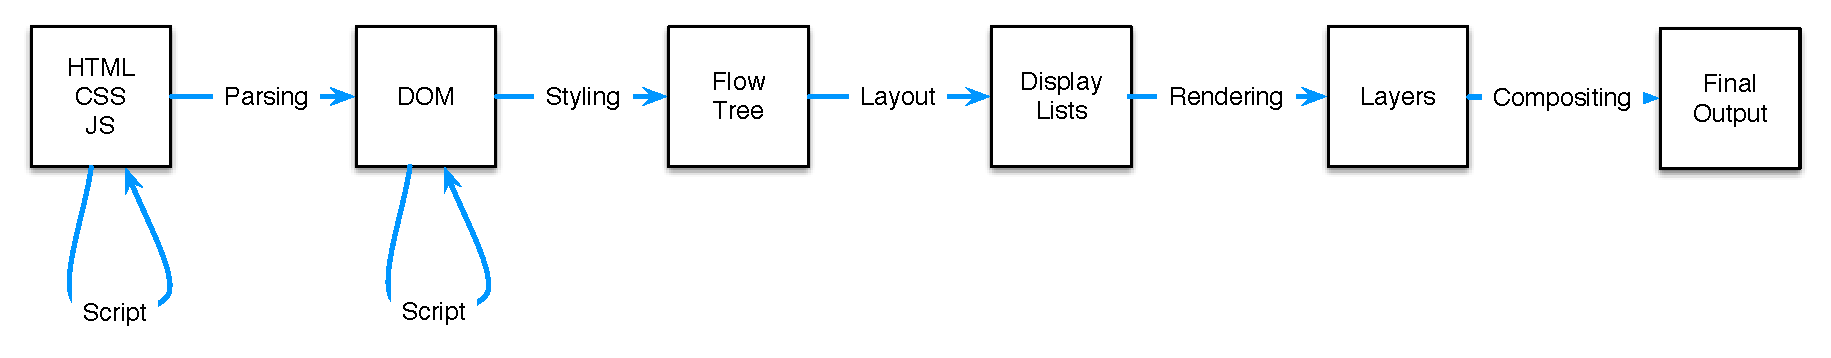
\includegraphics[scale=0.7]{pics/browser}
  \end{center}%
  \caption{Processing stages and intermediate representations in a browser engine.}
  \label{fig:browser}
\end{figure*}%

\subsection{Parsing HTML and CSS}

A URL identifies a resource to load.
This resource usually consists of HTML, which is then parsed and typically turned into a Document Object
Model (DOM) tree.
From a programming languages standpoint, there are several interesting aspects of the parser design
for HTML.
First, though the specification allows the browser to abort on a parse error\footnote{\url{https://html.spec.whatwg.org/multipage/#parsing}},
in practice browsers follow the recovery algorithms described in that specification precisely so that
even ill-formed HTML will be handled in an interoperable way across all browsers.
Second, due to the presence of the \lstinline[language=HTML]{<script>} tag, the token stream can be modified
during operation.
For example, the below example that injects an open tag for the header and comment blocks works in all modern browsers.
\begin{lstlisting}[language=HTML]
<html>
  <script>
  document.write("<h")\';
  </script>1>
  This is a h1 title

  <script>
  document.write("<!-");
  </script>-
  This is commented
  -->
</html>
\end{lstlisting}
This requires parsing to pause until JavaScript code has run to completion.
But, since resource loading is such a large factor in the latency of loading many webpages (particularly on mobile),
all modern parsers also perform speculative token stream scanning and prefetch of resources likely to be required~\cite{browsers-slow-smartphones}.

\subsection{Layout}

After constructing the DOM and determining the set of styles defined in the Cascading Style Sheets (CSS) that has
been loaded, those styles are applied to the DOM and a new flow tree that represents the elements is created.
This process can create many more flows than previously existed in the DOM --- for example, when a list item is
styled to have an associated counter glyph.

\subsection{Display}

That tree of elements, called the \emph{flow tree} in Servo, is then processed
to produce a set of \emph{display list} items.  These list items are the
actual graphical elements, text runs, etc. in their final on-screen positions.
The order in which these elements are displayed is well-defined by the
standard\footnote{\url{http://www.w3.org/TR/CSS21/zindex.html#painting-order}}.

\subsection{Rendering}

Once all of the elements to appear on screen have been computed, these
elements are rendered, or painted, into memory buffers or directly to graphics
surfaces.

\subsection{Compositing}

The set of memory buffers or graphical surfaces, called layers, are then
transformed and composited together to form a final image for
presentation.

\subsection{Scripting}

Whether through timers, \lstinline[language=HTML]{<script>} blocks in the
HTML, user interactions, or other event handlers, JavaScript code may execute
at any point during parsing, layout, and painting or afterwards during
display.  These scripts can modify the DOM tree, which may require rerunning
the layout and painting passes in order to update the output.  Most modern
browsers use some form of dirty bit marking to attempt to minimize the
recalculations during this process.


%%% Local Variables: 
%%% mode: latex
%%% TeX-master: "paper"
%%% End: 

%!TEX root = paper.tex

\section{Rust}
\label{sec:rust}

Rust is a statically typed systems programming language most heavily inspired by the C
and ML families of languages~\cite{RUST}.
Like the C family of languages, it provides the developer fine control over memory layout
and predictable performance.
Unlike C programs, Rust programs are \emph{memory safe} by default,
only allowing unsafe operations in specially-delineated blocks.

Rust features an \emph{ownership-based} type system inspired by the region systems work in the
MLKit project~\cite{mlkit} and especially as implemented in the Cyclone language~\cite{cyclone}.
Unlike the related ownership system in Singularity OS~\cite{singularity}, Rust allows programs to
not only transfer ownership but also to temporarily \emph{borrow} owned values, significantly
reducing the number of region and ownership annotations required in large programs.
The ownership model encourages immutability by default while allowing for controlled
mutation of owned or uniquely-borrowed values.

Complete documentation and a language reference for Rust are available at: \url{http://doc.rust-lang.org/}.

\subsection{Ownership and concurrency}
Because the Rust type system provides very strong guarantees about memory aliasing,
Rust code is memory safe even in concurrent and multithreaded environments,
but beyond that Rust also ensures \emph{data-race freedom}.

In concurrent programs, the data operated on by distinct threads is also itself distinct:
under Rust's ownership model, data cannot be owned by two threads at the same time.
For example, the code in \figref{fig:bad-concurrency} generates a static error from the compiler because
after the first thread is spawned, the ownership of \lstinline{data} has been transferred into the
closure associated with that thread and is no longer available in the original thread.
%http://is.gd/tkcD9R
\begin{figure}
\begin{lstlisting}
fn main() {
  // An owned pointer to a heap-allocated
  // integer
  let mut data = Box::new(0);

  Thread::spawn(move || {
    *data = *data + 1;
  });
  // error: accessing moved value
  print!(``{}'', data);
}
\end{lstlisting}
  \caption{Code that will not compile because it attempts to access mutable state from two threads.}
  \label{fig:bad-concurrency}
\end{figure}

On the other hand, the immutable value in \figref{fig:shared-concurrency} can be borrowed and shared between multiple threads as long as those threads don't outlive the scope of the data, and even mutable values can be shared as long
as they are owned by a type that preserves the invariant that mutable memory is unaliased, as with the
mutex is \figref{fig:shared-mutable-concurrency}.

\begin{figure}
\begin{lstlisting}
fn main() {
  // An immutable borrowed pointer to a
  // stack-allocated integer
  let data = &1;

  Thread::scoped(|| {
    println!(``{}'', data);
  });
  print!(``{}'', data);
}
\end{lstlisting}
  \caption{Safely reading immutable state from two threads.}
  \label{fig:shared-concurrency}
\end{figure}

\begin{figure}
\begin{lstlisting}
fn main() {
  // A heap allocated integer protected by an
  // atomically-reference-counted mutex
  let data = Arc::new(Mutex::new(0));
  let data2 = data.clone();

  Thread::scoped(move || {
    *data2.lock().unwrap() = 1;
  });

  print!(``{}'', *data.lock().unwrap());
}
\end{lstlisting}
  \caption{Safely mutating state from two threads.}
  \label{fig:shared-mutable-concurrency}
\end{figure}

With relatively few simple rules, ownership in Rust enables foolproof task parallism,
but also data parallism, by partitioning vectors and lending mutable references into properly scoped threads.
Rust's concurrency abstractions are entirely implemented in libraries, and though
many advanced concurrent patterns such as work-stealing~~\cite{blumeofe:multiprogrammed-work-stealing}
cannot be implemented in safe Rust, they can usually be encapsulated in a memory-safe interface.

%%% Local Variables: 
%%% mode: latex
%%% TeX-master: "paper"
%%% End: 

%!TEX root = paper.tex

\section{Language features}
\label{sec:lang}

%%% Local Variables: 
%%% mode: latex
%%% TeX-master: "paper"
%%% End: 

%!TEX root = paper.tex

\section{Affine types}
\label{sec:affine}

Compare with especially Singularity. Key point is having Servo and noticing that most APIs do not transfer ownership. By instead 'borrowing' the value, we do not have region types bleed into the interfaces, and avoid the major failure of Singularity.

%%% Local Variables: 
%%% mode: latex
%%% TeX-master: "paper"
%%% End: 

%!TEX root = paper.tex

\section{Unsafe code}
\label{sec:safety}

%%% Local Variables: 
%%% mode: latex
%%% TeX-master: "paper"
%%% End: 

%!TEX root = paper.tex

\section{Libraries and abstractions}
\label{sec:libraries}

%%% Local Variables: 
%%% mode: latex
%%% TeX-master: "paper"
%%% End: 

%!TEX root = paper.tex

\section{Open}
\label{sec:open}

%%% Local Variables: 
%%% mode: latex
%%% TeX-master: "paper"
%%% End: 

%!TEX root = paper.tex
%
\section{Conclusion}
\label{sec:concl}


\acks
The Servo project was started at Mozilla Research, but has benefitted from
contributions from Samsung, Igalia, and hundreds of volunteer community members.
These contributions amount to more than half of the commits to the project,
and we are grateful for both our partners' and volunteers' efforts to make
this project a success.


\bibliographystyle{../common/alpha}
\bibliography{../common/strings-short,../common/manticore}

\end{document}
